\documentclass[dvipdfm]{beamer}
\usepackage{graphicx}

\usepackage{xunicode}
\usepackage{xltxtra}
\XeTeXlinebreaklocale "zh"
\XeTeXlinebreakskip = 0pt plus 1pt
\setsansfont{Vera Sans YuanTi Mono}
\setromanfont{Vera Sans YuanTi Mono}

\usetheme{Warsaw} 
%\usecolortheme{seahorse} %sidebartab, rose
\title{学习计算机之心得与体会}
\author{盛艳 }
\institute{<shengyan1985@gmail.com>}
\date{2009 年 05 月 09 日} 

\begin{document}
\begin{frame}
  \titlepage
\end{frame}
% 各位同学下午好, 非常高兴能有机会来给大家做报告, 我想我能给在座的各位一些关于如何学习计算机, 如何掌握某一种技能, 如何学会学习的建议
% 和个人经验体会. 或者说, 如何从一只菜鸟变成一只老鸟? 希望能让大家有所启发或收获....不过, 首先申明,,,本人目前还是只菜鸟, 如果报告
% 过程中, 说的不对的地方, 欢迎随时指出. 我想更重要的是我们一起讨论, 交流, 这才是这次报告更有意义的东西.

\begin{frame}[t]{}
  \vspace{1em}
  \begin{center}
  
\includegraphics[height=8cm]{figure/www.eps}
  \end{center}
\end{frame}
% 首先, 目前的网络发展速度是比我们想象中的速度还要快, 互联网连接整个世界, 而上面的信息资源每时每刻都在急剧增加, 对于计算机相关的
% 新的技术, 新的知识, 新的东西, 我们该如何面对, 如何去接受, 去学习这么多的新知识呢? 我想, 只要掌握了学习的真正方法, 那不管以后学
% 任何新的东西, 都能很快上手. 下面就讲述些在学习成长过程中, 非常重要的几个东西.

\begin{frame}[t]{兴趣}
  \begin{block}{兴趣第一}
    \begin{itemize}
    \item  产生兴趣 \pause
    \item  发现自己 \pause
    \item  培养自己 \pause
    \item  好奇, 多问为什么 \pause
    \item  寻找 \pause
    \item  实践
    \end{itemize}
  \end{block}
\end{frame}
% 兴趣永远是第一位的, 因为你有了兴趣才能让你有继续了解, 深入学习它的机会. 可能刚开始, 会觉得计算机东西太多太杂, 
% 日新月异的技术发展似乎已经超出我们的接受能力, 又或者是, 编程太枯燥乏味, 导致我们很多时候什么都不想做. 不想看书, 不想写代码等等,
% 这是为什么? 其中很大个原因, 是由于你没有在获取知识的过程中体会到乐趣, 你没有对她产生兴趣. 那么, 我们该怎么样呢? 
% 首先, 发现自己, 真正了解自己的爱好 , 并时刻关心某方面的东西.
% 其次, 培养自己, 锻炼自己, 从具体的应用中加强自己对某方面的认识.
% 最后, 自己要有一颗好奇的心, 碰到一些事情, 多问问为什么, 这个东西是用来做什么的, 为什么这样做等等 
% 我举个例子, 比如说, 我小时候喜欢画画, 但现在有了计算机, 计算机中就能进行图像处理 , 而且功能强大. 在网上找找相关工具, 一大堆.
% PS, Illustrator, CoralDraw, Picasa等等. , 我们就通过一些工具来完成图片处理. 这样我们就有了学习她的兴趣...就是我喜欢制作
% 效果非常酷的图片. 在当你熟悉了某个现有工具的使用之后, 你会觉得她的某个功能不好, 不符合我的需要, 那我会怎么做呢,,,,一种方式是寻找
% 其他的图片处理软件, 看她是否有这样的功能, 这样的话, 你就需要熟悉另外一个工具,,,另外一种就是, 深入的理解图片处理知识, 看现有的
% 图片处理工具是怎样进行处理的, 比如说, 如何读取一图片, 如何区分不能图片格式, 如何加亮一副图片. 这些问题都可以在你查找网上资料,
% 翻阅相关书籍后找到答案. 既然知道了里面的机理是怎样的, 那么我们需要实践, 把它实现出来, 就能更好的加深印象. 而且你能在这个过程中,
% 发现更多的问题, 也就是说在你解决某个问题之后, 又会有新的问题发现等待着你去解决, 在这样的不断发现问题, 解决问题的过程中, 你会学到
% 更多的东西. 哪天你会不知不觉得发现自己知道的东西变得广泛了许多.
% 

\begin{frame}[t]{目标}
  \begin{block}{给自己设定一个目标}
    \begin{itemize}
    \item 选择是痛苦的 \pause
    \item 但如果目标坚定, 你会很容易作出选择 \pause
    \end{itemize}
  \end{block}
  \begin{center}
  \centering 
\includegraphics[height=6cm]{figure/goal.eps}
  \end{center}
\end{frame}
\begin{frame}[t]{目标}
  \begin{block}{给自己设定一个目标}
    \begin{itemize}
    \item 坚持不懈 \pause
    \end{itemize}
  \end{block}
  \begin{center}
  \centering 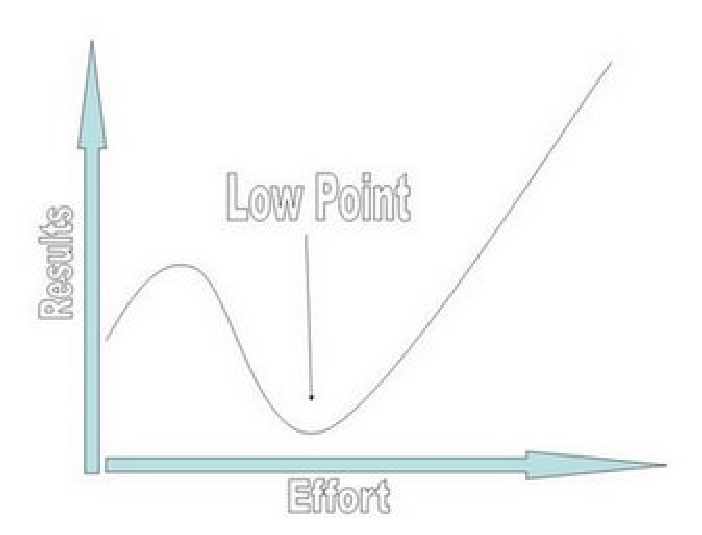
\includegraphics[height=6cm]{figure/effortandresult.eps}
  \end{center}
\end{frame}
% 其实, 我们每天都在做各种各样的选择, 选择今天早上是请病假窝在宿舍睡懒觉还是去冷冰冰的教室上自习? 选择今天是看电影, 玩游戏, 还是看点书?
% 选择这学期就这样混过去, 只求考试60分万岁, 还是认认真真理解基础知识, 掌握各种精华? 这些都是自己的选择...
% 选择是和你的目标紧密联系在一起的, 如果目标明确了, 自然会很容易的作出选择. 这个涉及到个人心态, 价值观, 人生观问题, 我也不便多说什么,
% 各位可以好好体会下, 可能现在不理解, 体会不了, 但随着时间的推移, 我相信你会慢慢体会的了的.
% 不管怎样, 想说明的一点就是, 明确自己的目标, 短期目标, 长期目标是什么? 如果有, 就要坚定这个目标, 并不断坚持不懈的努力下去; 
% 如果没有, 那么从现在开始, 好好想想清楚, 给自己定个目标.
% 有这样一幅图说明了一项新的兴趣的付出和回报的曲线关系, 足以说明咱们做感兴趣的事情时, 往往会先开始进展神速, 随后就会进入瓶颈, 此时可能会变得没有兴趣, 但是凭借毅力坚持下来, 你就会变得越好越好. 咱们周围的很多事情似乎都是这样的, 回想自己当初对研究的热爱, 似乎也是这样一种曲线关系.

\begin{frame}[t]{其他}
  \begin{block}{其他的几点建议}
    \begin{itemize}
    \item 扎实基础
    \item 勤作笔记, 总结
    \item 慢慢积累, 注重过程
    \item 开放视野
    \end{itemize}
  \end{block}
\end{frame}
% 刚才那两点, 是我觉得最最最重要的, 所以讲得比较多, 而以下的几点, 是我平时总结出来的几条, 可以说是心得体会吧. 
% 扎实基础, 不要以为书上的关于计算机的基础知识真的没有什么用处. 因为在很多地方, 你会发现最原始的, 最底层的东西还是很重要, 
% 而且也相对来说不会有多少变化. 
% 勤作笔记, 总结, 这是一个复习的过程, 相信我,,,作笔记比光光用眼睛看某些东西, 你的印象会更深刻...如果觉得写在纸上的笔记会让写的手酸的话, 
% 建议可以写在计算机上, 更好的就是, 比如写一个博客, 专门用来记录自己学到的东西, 或者一些问题, 一些体会. 这在给自己加深印象的同时, 
% 也可能会无意间给别人一些帮助, 当哪天某人专门发邮件给你问你博客文章上的某个问题时, 到时你会觉得很有价值感, 我相信你一定会无比高兴的.
% 慢慢积累, 注重过程, 很多你拥有的东西是依靠你现在一点一滴的积累起来的.
% 开放视野, 尽量接收更多更新的讯息, 常常关注些新的技术, 新的发展趋势.

% 这些只是我这么多年总结出来的一些经验, 可能有些东西还是需要自己慢慢的体会的, 可能也有些东西不适用大家.
% 下面还有些时间, 我想和大家介绍一些新颖的技术. 不知道大家对计算机和网络的哪些方面感兴趣呢?


\begin{frame}[t]{有意思的东西}
  \begin{block}{FriendFeed}
    \begin{itemize}
    \item 集成各种服务, 如博客, 照片, 书签, 微博, 新闻, 视频, 音乐等等, 朋友间可以相互订阅以便能获得最新的讯息. 类似的还有, drop.io, chi.mp等等 
    \end{itemize}
  \end{block}
  \begin{center}
  \centering 
\includegraphics[height=4cm]{figure/ff.eps}
  \end{center}
\end{frame}

\begin{frame}[t]{有意思的东西}
  \begin{block}{twitter}
    \begin{itemize}
    \item 微博, 开放api, 多种客户端, 信息传递迅速. 类似的有, 饭否, 叽歪等
    \end{itemize}
  \end{block}
  \begin{center}
  \centering 
\includegraphics[height=6cm]{figure/twitterw.eps}
  \end{center}
\end{frame}

\begin{frame}[t]{有意思的东西}
  \begin{block}{在线编辑}
    \begin{itemize}
    \item 在线编辑图片, 如FlauntR, Picnik, Scrapblog等等 \pause
    \end{itemize}
  \end{block}
  \begin{center}
  \centering 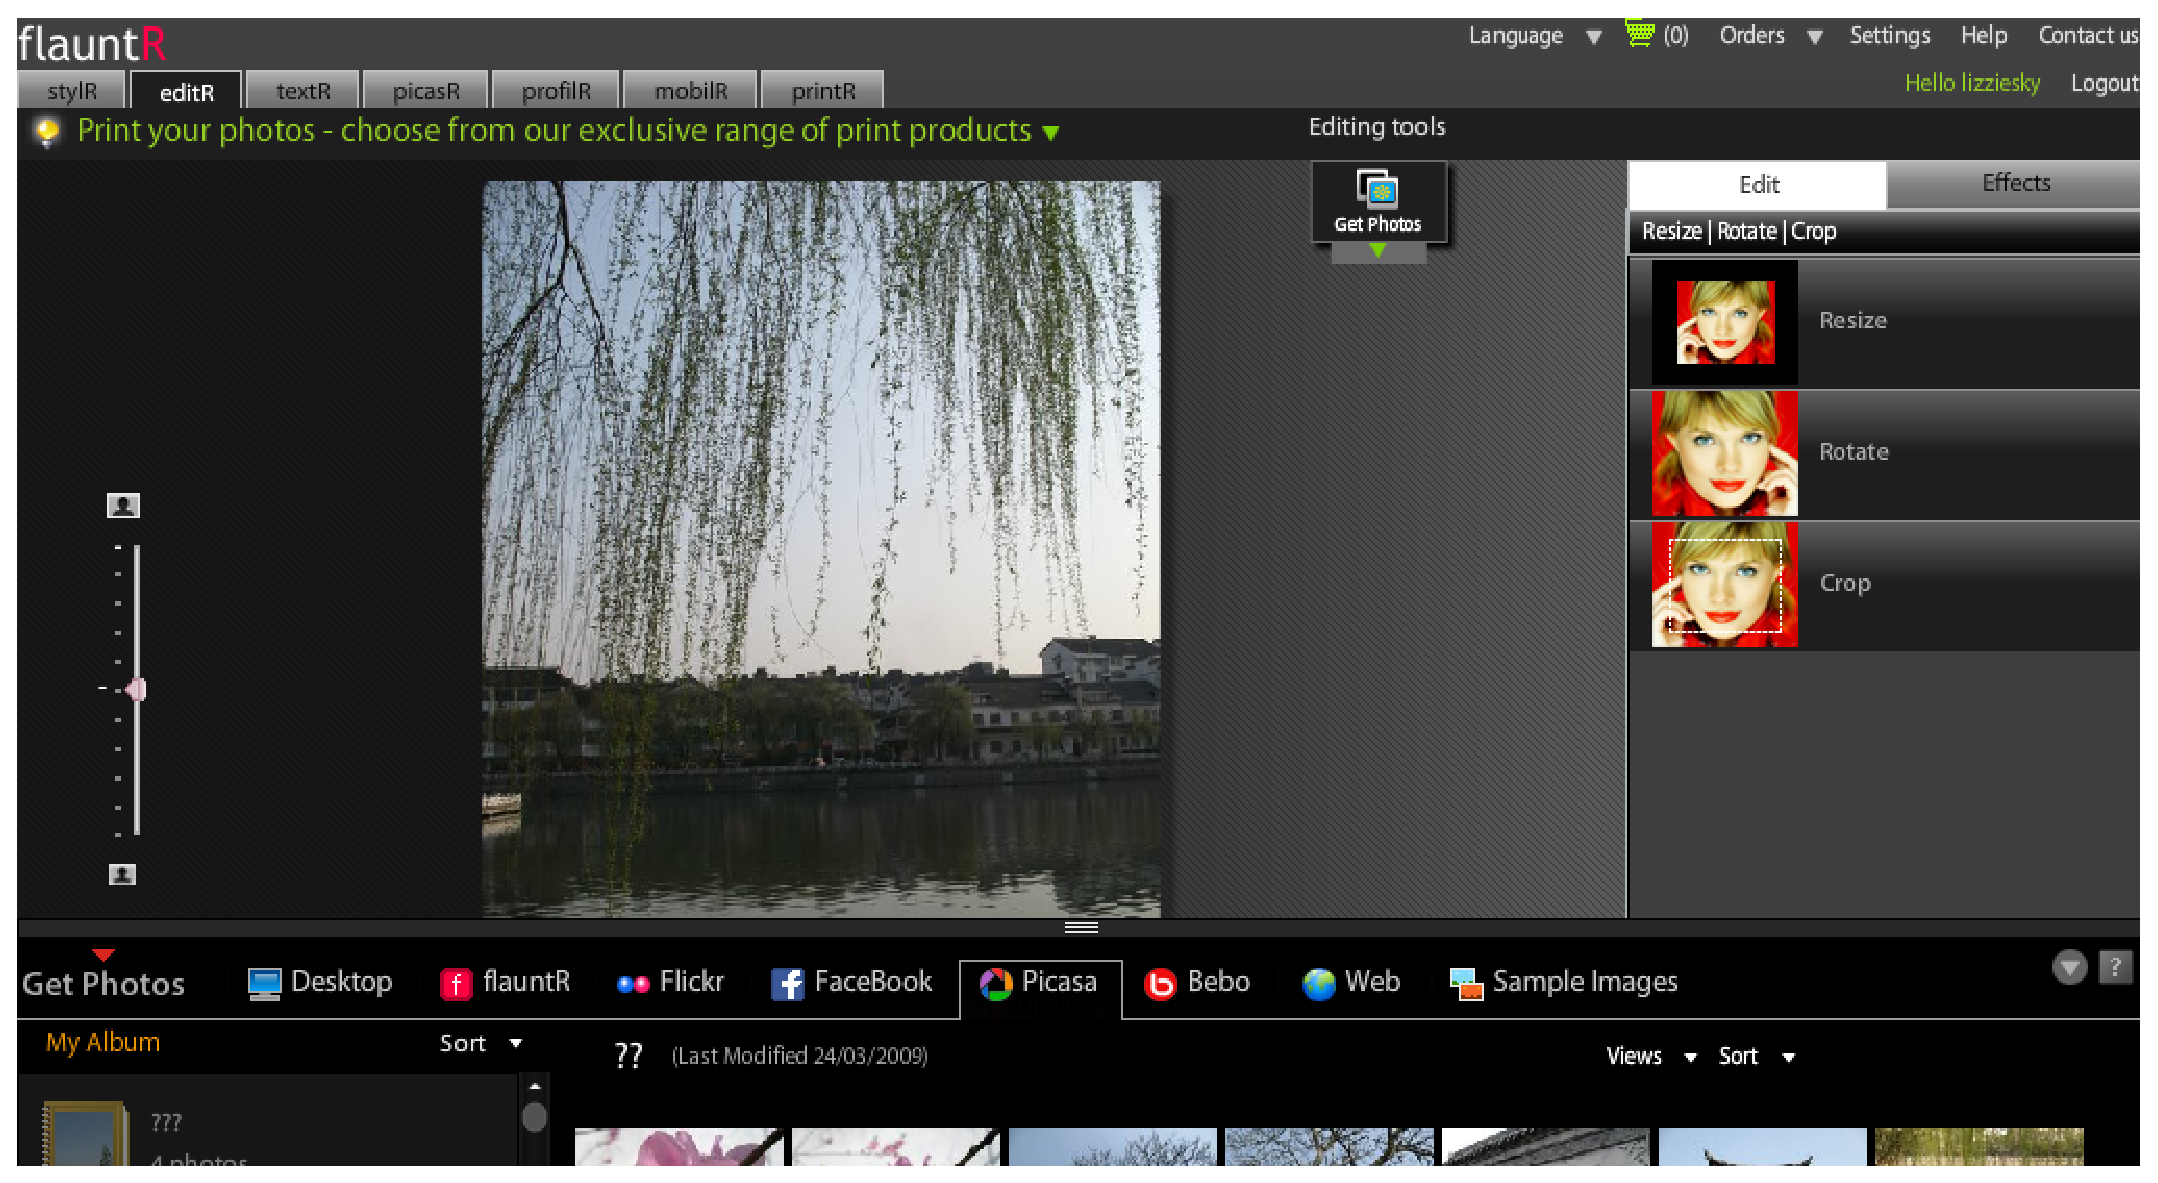
\includegraphics[height=6cm]{figure/flauntr.eps}
  \end{center}
\end{frame}

\begin{frame}[t]{有意思的东西}
  \begin{block}{O3D}
    \begin{itemize}
    \item 开源的web API, 用于在浏览器中创建丰富的, 可交互的3D应用.  \pause
    \end{itemize}
  \end{block}
  \begin{center}
  \centering 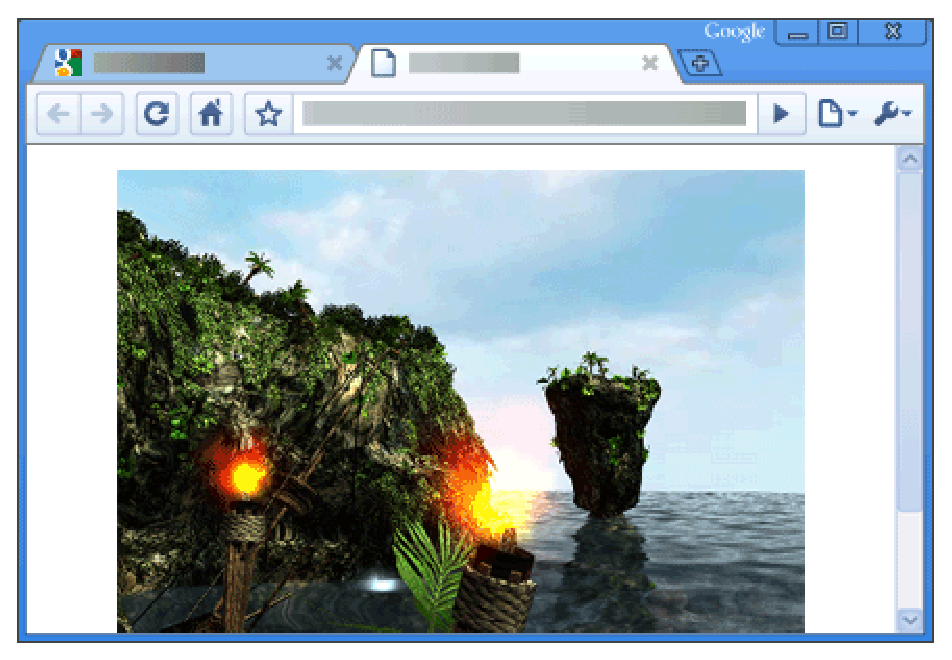
\includegraphics[height=6cm]{figure/o3d.eps}
  \end{center}
\end{frame}

\begin{frame}[t]{有意思的东西}
  \begin{block}{可视化搜索}
    \begin{itemize}
    \item 提供多种形式的搜索结果展示, 比如有viewzi, searchme.  \pause
    \end{itemize}
  \end{block}
  \begin{center}
  \centering 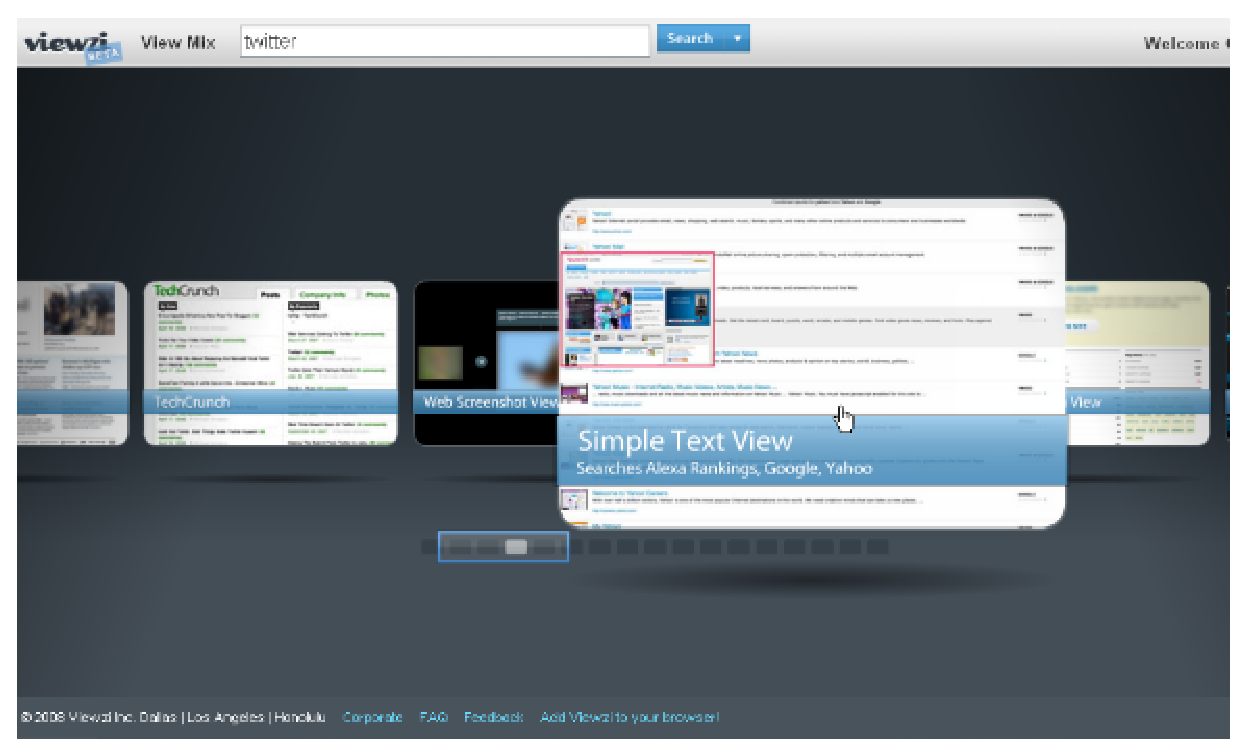
\includegraphics[height=6cm]{figure/viewzi.eps}
  \end{center}
\end{frame}

\begin{frame}[t]{经常用的Web service}
  \begin{center}
  \centering 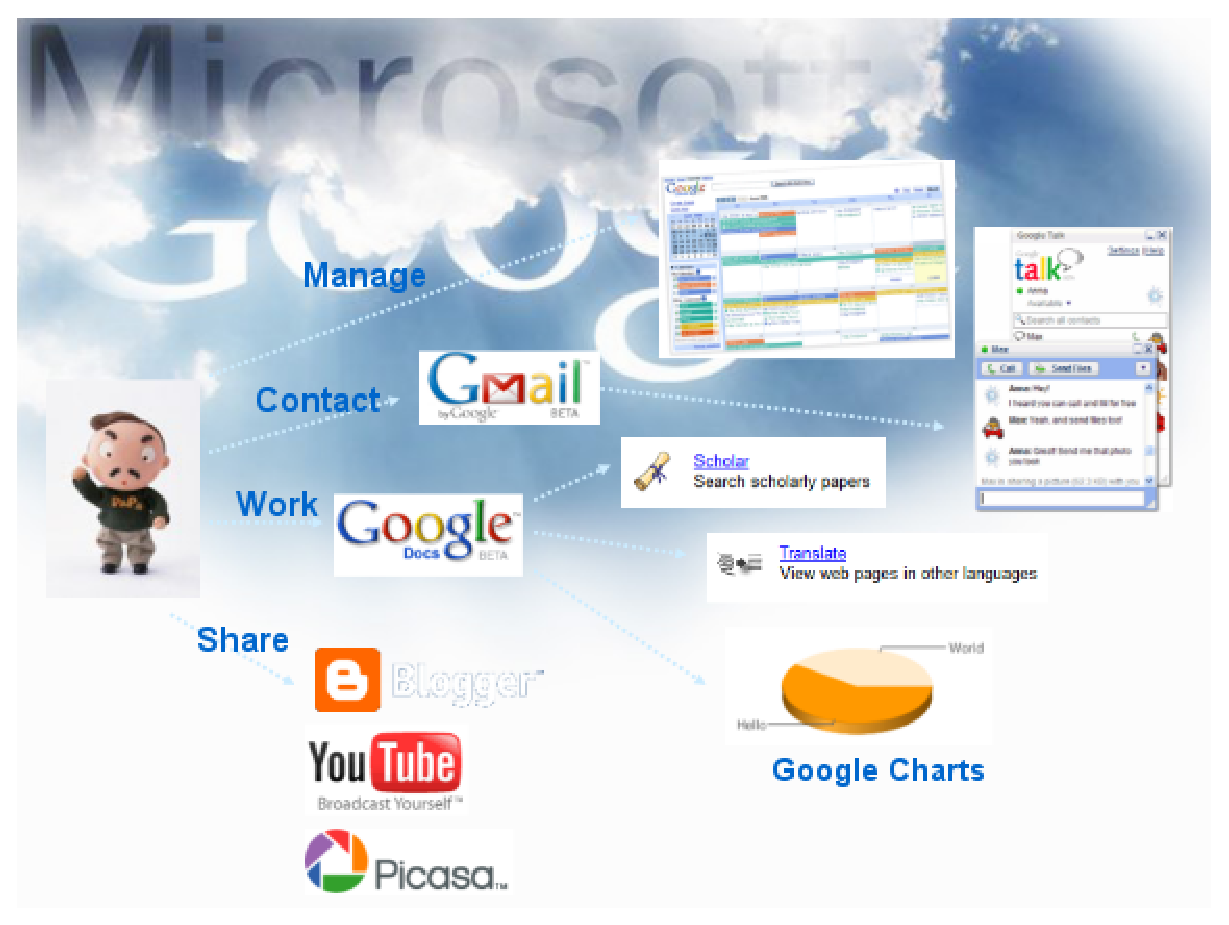
\includegraphics[height=8cm]{figure/ws.eps}
  \end{center}
\end{frame}

\begin{frame}[t]{经常用的Web service}
  \vspace{1em}
  \begin{center}
  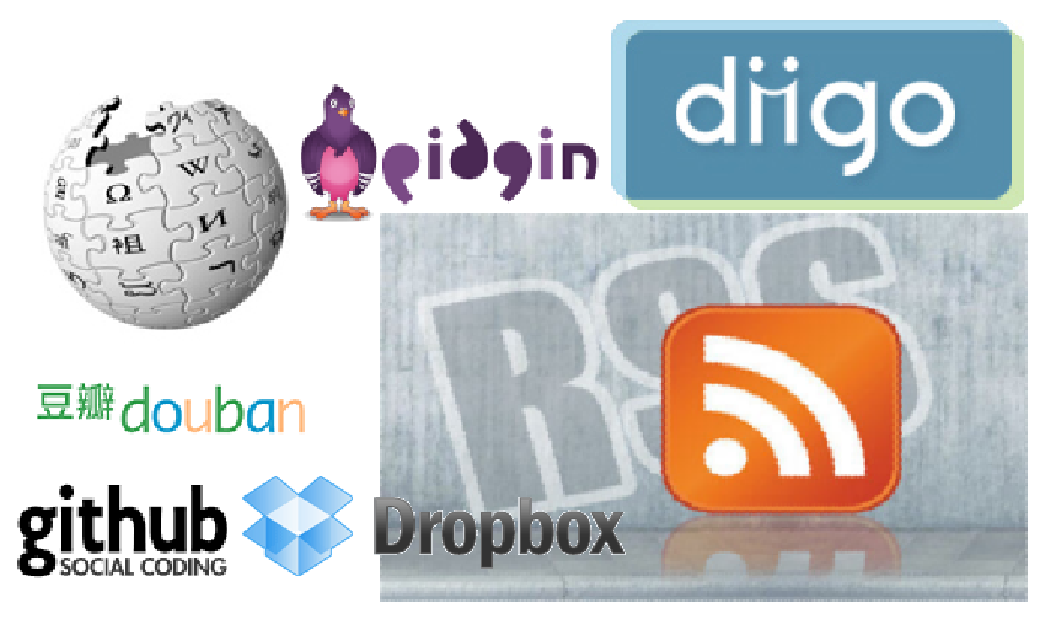
\includegraphics[height=6cm]{figure/ws2.eps}
  \end{center}
\end{frame}

\begin{frame}[t]{最后一点提醒}
  \begin{center}
  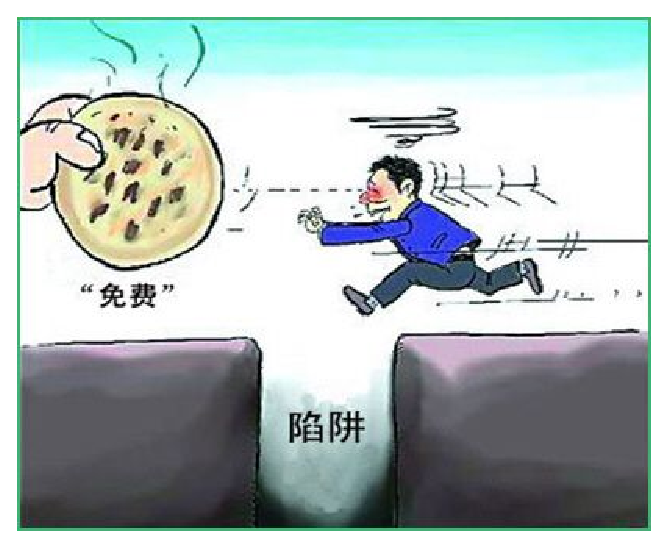
\includegraphics[height=7cm]{figure/warning.eps}
  \end{center}
\end{frame}
% 互联网还是不可信任的, 我们需要时刻提醒自己这点. 所谓提供的免费服务, 想想它们为何要提供给你.
% """即便在互联网上, 我最信任的企业是Google, 然而我并不希望当我准备出门时, Google会发来一封邮件提醒我带雨伞, 因为第二天会下雨. """

% 致谢 非常高兴能和各位同学一起讨论交流
\begin{frame}[t]{...}
\vspace{5em}
\begin{center}
\Huge{谢谢大家!}
\end{center}
\end{frame}

\end{document} 
